%12/03 - Enrique Carrillo
\part{Regulación Genómica y Epigenómica}
\chapter{Introducción y regulación genómica}
\section{Avances impulsados por el Proyecto Genoma Humano}
El coste del proyecto genoma humano fue equivalente a mandar el hombre a la Luna, por lo que tuvo un gran impacto a nivel global y de humanidad. Cambió la visión de la biología. 
Entre los avances se encuentran:
\begin{itemize}
\item Datos democratizados, públicos, disponibles gratuitamente online a la información.
\item Mapa genético y físico: alrededor de 21.000 genes y conocemos su localización en el genoma, aún más sus interacciones 3D
\item Desarrollo de nuevas tecnologías: secuenciación
\item Identificación genética: conocemos el mapa de posición y rastreamos las consecuencias de las variaciones.
\item Aplicación de técnicas bioinformáticas y de machine learning
\end{itemize}

Nota rápida: Margaret Oakley Dayhoff fue la pionera en el campo de la bioinformática. Dedicó su carrera a la aplicación de tecnologías computacionales en biología y medicina, principalmente mediante la creación de bases de datos de proteínas y ácidos nucleicos, así como de herramientas de acceso a historias cortas.

Luego se vivió la revolución de la secuencia del genoma humano. Se desarrollaron muchos proyectos de cáncer, transcriptómica, aumento de las bases de datos, etc. 

\section{Regulación genómica}
La regulación genómica controla cuándo, dónde y cuánto se expresan los genes.

\subsection{Estructura del ADN y elementos reguladores}
Siendo muy simplista, el ADN se divide en la hebra simple, que se empaqueta con las histona hasta llegar al cromosoma completamente compactado. La regulación va de esto: cómo se empaqueta y desempaqueta el ADN para que se produzcan distintos sucesos (la transcripción fundamentalmente). 

Los genomas son muy complejos, ya que más de 10x y 30x del ADN es necesario para codificar proteínas. Los genomas se pueden clasificar en regiones codificantes (exones) y regiones no codificantes, entre los que se encuentran intrones, regiones intergénicas, regiones reguladoras (promotores, potenciadores, regiones silenciadoras, insulators, generalmente relacionados con la actividad de los factores de transcripción), pseudogenes (relacionados con genes pero que han perdido actividad debido a un proceso mutacional), regiones repetitivas (regiones satélite, retrotransposones, SINE, LINE, ...) y regiones transcritas no codificantes (miRNA, siRNA, piRNA, lncRNA). Éstos últimos se analizan como si fueran datos transcriptómicos, cuantificándolos. 

Entre los elementos reguladores destacan:
\begin{itemize}
\item Promotores: regiones que inician la transcripción mediante TATA box, CAAT box, GC box
\item Enhancers: aumentan la expresión de genes distantes. Esto es muy complicado de encontrar en la inmensidad del genoma al no estar caracterizados.
\item Silencers: reprimen la transcripción de genes distantes. También son difíciles de caracterizar computacionalmente. 
\item Insulators: aíslan regiones para prevenir efectos reguladores no deseados. Estas regiones están asociadas a determinadas proteínas. 
\end{itemize}

Un gen empieza por un promotor y tiene distintos exones e intrones. El gen termina en una señal de poliadenilación. Las regiones promotoras son segmentos del ADN que precede los sitios de iniciación de los sitios de transcripción (transcription start site). Esta región atrae la ARN polimerasa.

\subsection{Predicción de genes y motivos de ADN}
Existen regiones del ADN con secuencias que permiten predecir la presencia de genes, como el transcription start site. Ahora mismo ya no es un gran reto porque hay muchas bases de datos sobre esto (por ejemplo, \href{http://epd.vital-it.ch}{EPD}), pero se utiliza mucho en el laboratorio, teniendo que hacer un fine-tuning. 

Los estudios CAGE capturan los inicios de la transcripción de forma experimental. Se marca el inicio del ARN mensajero con un cap para seguirlo y detectarlo. FANTOM es un buen recurso para asignar anotaciones funcionales a los tránscritos. 

\subsection{Detección de enhancers}
Los enhancers son complicados desde el punto de vista bioinformático al tener varias conformaciones distintas. Además, como pueden estar lejos en el espacio, no conocemos la distancia concreta. Otras veces se necesitan varios factores de transcripción hasta llegar a unirse a la polimerasa en el promotor, y en otras ocasiones se forma un loop. Aquí no hay números, por lo que su estudio es complejo. Pero como esto es lo que más regula la expresión de los genes, es un campo en auge. 

No siempre es 1 enhances - 1 gen, si no que puede haber 1 enhancer para varios genes, afectándolos de formas distintas, aumentando su complejidad. Si sabemos que unas proteínas necesitan un determinado enhancer, con datos de ChIP-Seq sí se podría localizarlos.

Con los silenciadores, el concepto es el mismo, pero con el efecto contrario. 

Por convenio, se buscan promotores en 1 kilobase, pero la decisión está en el bioinformático. No es lo mismo decidir 1 kb que 5 kb, y esta decisión afecta posteriormente al análisis de enriquecimiento. 

\subsection{Motivos de unión a factores de transcripción}
Los factores de transcripción se unen al promotor para afectar al gen. Estos factores tienen motivos concretos de unión, lo cual facilita el análisis al poder escanear todo el genoma en busca de ese motivo. Pero hay varios problemas:
\begin{itemize}
\item Consensos a menudo mal definidos, no siempre son perfectos al poder cambiar alguna base, tener una base más o menos.
\item Secuencias no conservadas dentro de las especies, y peor aún entre especies, por lo que no vale buscar el motivo en una especie para aplicarlo en otra.
\item Ejemplos de enhancers conservados funcionalmente pero no conservados en su secuencia, por lo que encontrar motivos de unión puede ser complicado.
\item La mayoría de los datos de secuencias de TFBS proceden de unas pocas especies: ratón, humano y poco más.
\item Muy a menudo son experimentos \textit{in vitro}, pero poco a poco está aumentando ChIP-Seq.
\item 2 sitios de unión completamente diferentes podrían fusionarse en la misma matriz/consenso. 
\end{itemize}

Una matriz tiene una fila para cada secuencia y una columna para cada posición. Se cuentan así las bases para cada posición, calculando el consenso. Gracias a estas matrices se pueden buscar los motivos en el genoma. Esto se puede representar después con logos, en el que el contenido de información de la columna de una matriz va desde 0 hasta 2. 

Bases de datos a utilizar es TRANSFAC, pero es de pago. No obstante, hay programas que pagan para poder utilizar la base de datos dentro, por lo que es una de las más utilizadas. Esta base de datos tiene un score de calidad:
\begin{enumerate}
\item Sitio de unión al factor de transcripción confirmado funcionalmente
\item Unión de proteína pura (purificada o recombinante)
\item Actividad de unión caracterizada inmunológicamente de un extracto celular
\item Actividad de unión caracterizada mediante una secuencia de unión conocida
\item Unión de proteína de extracto no caracterizada a un elemento de buena fe
\item Sin calidad asignada
\end{enumerate}

Otra base de datos es JASPAR. Permite elegir los factores de transcripción y sus matrices, la especie, etc. 

\subsubsection{Ejercicio}
Nos vamos a Ensembl y nos descargamos la región codificante del gen BRCA2. Una vez en Jaspar, en la búsqueda seleccionamos el genoma humano y seleccionamos todos los factores de transcripción. A la derecha hay varias opciones y debemos seleccionar Scan. Pegamos la secuencia en FASTA y podemos especificar el umbral de puntuación del perfil relativo. 

\subsection{Descubrimiento de patrones}
Es posible encontrar motivos desconocidos mediante el análisis del genoma completo, clusterizando y realizando análisis. Además, se pueden realizar estadísticas como frecuencia esperada y observada. A veces no es necesario coger el genoma completo. Por ejemplo, para analizar solo enhancers, se puedes coger regiones que ya se han establecido como enhancers. Hay programas que no lo permiten, pero en otras ocasiones se puede especificar o poner una "black list". 

Los factores de transcripción pioneer se unen a determinadas regiones para estirar el ADN y liberar los genes para su transcripción. Estos son difíciles de trabajar, ya que se unen a zonas con nucleosomas, siendo complicado establecer sus motivos de unión. Al recibir un fichero con datos de ChIP-Seq de estos factores de transcripción, es importante conocerlo para adaptar el análisis. 

Otras herramientas útiles son:
\begin{itemize}
\item MEME-Suite: tiene muchas herramientas para identificar secuencias, clusterizar, etc.
\item HOMER Motif Analysis: sirve para motivos de unión, pero también Hi-Seq, análisis funcional, etc.
\item RSAT: está separado en hongos, procatriotas, plantas, etc.
\item TRAP
\end{itemize}

\subsubsection{Ejercicio}
Desde GEO, nos descargamos los picos del experimento GSE47535 y eliminamos la primera línea. Convertimos el BED en FASTA y lo analizamos con Meme-Suite. 


\chapter{Epigenética}
La epigenética se ha definido de muchas maneras a lo largo del tiempo. Primero fue el estudio entre la interacción entre genes y el ambiente. Posteriormente fue el estudio de los mecanismos que controlan la actividad de los genes durante el desarrollo. En el 2009 ya se definió como el estudio de los fenotipos hereditarios resultantes de cambios cromosómicos sin alteraciones en la secuencia del ADN. Ahora se podría definir como el estudio de la organización cromosomal y la regulación de la actividad genómica sin cambio nucleotídico. 

La genética estudia la secuencia primaria del ADN y sus cambios, mientras que la epigenética estudia la modificación química en el ADN y proteínas asociadas sin cambios de secuencia. En un nucleosoma hay 8 histonas, y se buscan cambios químicos en el ADN y las histonas. También puede haber distintas conformaciones de las histonas. Lo más importante son las colas de las histonas, ya que es donde se darán los cambios. 

\section{Mecanismos epigenéticos}
Hay fundamentalmente cuatro mecanismos epigenéticos:
\begin{itemize}
\item Modificación de histonas
\item Cambios de composición de histonas
\item Modificaciones de citosina
\item Interacción de modificadores de cromatina
\end{itemize}

\subsection{Modificaciones de histonas}
Hay varias, pero las principales son acetilación, metilación, ubiquitinación, sumoylación y fosforilación. Las modificaciones se han asociado a distintas funciones. Es importante saber con qué tipo de histonas se trabajan y qué residuos de las colas pueden tener esas modificaciones. También hay que saber la anotación: H3K27me3 significa que en la histona 3, en la lisina 27 hay una triple metilación. 

Las modificaciones de las histonas se van a combinar entre ellas, por lo que el análisis se puede complicar. Las modificaciones tienen distintas acciones: escribir cosas, borrar o leer. Algunas modificaciones son compatibles, mientras que otras son incompatibles. En estudios en bulk, las pequeñas diferencias son importantes al poder indicar pequeñas subpoblaciones. Algunas modificaciones de histonas se han relacionado con enhancers unirse con factores de transcripción. 

Muchas de las histonas están ya estudiadas y tienen unos perfiles conocidos. Esto ayuda a la hora de analizar un perfil para saber qué esperamos. Las histonas son mecanismos generales, no específicos, teniendo que salir perfiles iguales. Para histonas activadoras, la densidad es muy superior al background. El problema está con las histonas inhibidoras, ya que la densidad es similar al background. Las señales no son tan grandes, y los peak callers funcionan muy mal en general, teniendo que utilizar log ratio. 

\begin{figure}[h]
\centering
\includegraphics[width = 0.9\textwidth]{figs/histone-modification.png}
\includegraphics[width = 0.7\textwidth]{figs/1-s2.0-S0968000410000940-gr1.jpg}
\end{figure}

%14/03 - Enrique Carrillo
Como cada vez aumenta la capacidad computacional, la cantidad de muestras también aumenta. Hay estudios con 10.000 mapas epigenómicas de 800 muestras. Esto permite ver las modificaciones de histonas en distintos tipos celulares y tejidos. 

Epimap es un repositorio de mapas epigenéticos de 15.000 datasets. 

\subsection{Cambios en la composición de histonas}
Las histonas se detectan con anticuerpos o ChIP-Seq. Se han estudiado las distintas combinaciones de las histonas que tienen funciones distintas. Para el ChiP-Seq, se utilizan anticuerpos que se unen a la histona. Mediante DNAsas se recorta el ADN y se libera el anticuerpo. En estos experimentos se necesita un control para evaluar los picos. Esto habitualmente se hace igual, pero sin anticuerpo. Las densidades de las secuencias se mapean y se compara cómo de denso es el pico frente al control. 

Las modificaciones de la cromatina coexisten en regiones genómicas. Por ello se han generado distintos modelos:
\begin{itemize}
\item Modelo combinatorio: Combinación de modificaciones específicas de las histonas que codifica
\item Modelo aditivo: La suma de los efectos individuales de las modificaciones de las histonas
que contribuye a la estabilidad y robustez.
\end{itemize}

\section{Métodos de segmentación}
El objetivo es combinar las distintas modificaciones de las histonas para detectar diferentes estados funcionales de la cromatina en todo el genoma. Se quieren revelar elementos funcionales sin tener que mirar la secuencia. De esta forma, se puede aprender \textit{de novo} patrones espaciales y combinatorios de marcas de cromatina. También se utiliza mucho para anotar genes. 

Una herramienta para esto es ChromHMM. Las histonas tienen dos estados: datos conocidos (los picos en el genoma) y los datos no conocidos (estados de cromatina). La herramienta utiliza los modelos ocultos de Markov.

Se crean ventanas del genoma de 200 pares de bases. Con estos fragmentos se calculan enriquecimientos individuales de cada modificación de histona (presencia o ausencia, binario). Se entrena un modelo de Machine Learning con todas las modificaciones de histonas y tipos celulares al mismo tiempo. Algo no resuelto es la cantidad de estados que hay que entrenar, por lo que hay que probar. La recomendación genera es definir los estados como el mínimo número de variables con interpretación biológica. Se intenta anotar con ayuda de datos externos como RefSeq o distancia a TSS, CpG, etc. Una vez con el modelo creado, se utiliza el genoma de las muestras y se segmenta el genoma de las muestras para ver el estado de cada una de las ventanas. Si algunos estados son muy similares, se pueden agrupar a posteriori. 

\subsection{Determinación de Estados de Cromatina a partir de Datos de ChIP-Seq}
Nos descargamos ChromHMM. Funciona tanto en Linux como en la CMD de Windows. En el directorio con el programa, ponemos \texttt{java -mx1600M -jar ChromHMM.jar LearnModel SAMPLEDATA\_HG18 OUTPUTSAMPLE 10 hg18}, y se debe ejecutar y crear un webpage\_10.html. Ahora nos vamos a descargar los datos. Para la práctica, se nos han facilitado los ficheros ya procesados, pero habría que descargarlos (\texttt{wget wgEncodeBroadHistoneMonocd14ro1746*AlnRep*.bam}), eliminar duplicados (\texttt{samtools rmdup –s <file>.bam <file>\_RM.bam}), convertir bam a bed (\texttt{bamToBed –i <file>\_RM.bam > <file>\_RM.bed}). 

En la carpeta CHROMSIZES creamos un fichero hg19\_chr16.txt y escribimos chr16 90354753 separado por tabulador. Ahora debemos crear file config\_chromHmm\_bin.txt como se indica en el manual:
\texttt{cell1 mark1 cell1\_mark1.bed cell1\_control.bed} separado por tabuladores.

%26/03 - Enrique
El siguiente paso es binarizar los datos en ventanas de longitud 200pb. 
\texttt{java -jar ChromHMM.jar BinarizeBed -c ./input/
./CHROMSIZES/hg19\_chr16.txt ./archivos/
config\_chromHmm\_bin.txt ./RESULTS}

Ahora vamos a entrenar modelos HMM para los distintos estados. No conocemos los estados, por lo que entrenamos varios para ver cuál es el mejor. Empezamos por un modelo con 8 estados y repetimos para 9-11:
\texttt{java -jar ChromHMM.jar LearnModel -i Master\_8 -l ./CHROMSIZES/hg19\_chr16.txt -printposterior -printstatebyline ./RESULTS ./RESULTS/LearnModel\_8 8 hg19}

\texttt{java -jar ChromHMM.jar LearnModel -i Master\_9 -l ./CHROMSIZES/hg19\_chr16.txt -printposterior -printstatebyline ./RESULTS ./RESULTS/LearnModel\_9 9 hg19}

\texttt{java -jar ChromHMM.jar LearnModel -i Master\_10 -l ./CHROMSIZES/hg19\_chr16.txt -printposterior -printstatebyline ./RESULTS ./RESULTS/LearnModel\_10 10 hg19}

\texttt{java -jar ChromHMM.jar LearnModel -i Master\_11 -l ./CHROMSIZES/hg19\_chr16.txt -printposterior -printstatebyline ./RESULTS ./RESULTS/LearnModel\_11 11 hg19}

Abrimos por ejemplo el report website\_11\_Master\_11.html. El primer heatmap representa los estados con las marcas epigenéticas. Después hay un plot de transición de estados, en el cual se representa la probabilidad de pasar de un estado a otro contiguo. 

Entre los archivos resultantes, se ha generado un txt con el modelo generado. Esto es muy útil si recibimos muestras nuevas con las mismas marcas epigenéticas, ya que no es necesario volver a ejecutar todo. No obstante, si hubiese alguna marca nueva no incorporada en el modelo, sí habría que replicar el procedimiento anterior.

Cuando hay replicados, se puede crear una regla en la que nos quedemos con regiones en las que x replicados muestren un mismo estado para poder definir la región a nivel biológico. En otros casos, tenemos un solo replicado. Como referencia, nos podemos quedar con aquellos estados con una probabilidad posterior mayor del 0.95. 

Ahora hay que comparar los modelos. Creamos una carpeta Compare en la que copiamos los ficheros emissions.txt de los cuatro modelos ahí. Ahora ejecutamos el siguiente comando:

\texttt{java -jar ChromHMM.jar CompareModels ./RESULTS/LearnModel\_11/emissions\_11\_Master\_11.txt
./RESULTS/Compare/
./RESULTS/Compare/Model\_compared}.

%02/04 - Enrique
\section{Epigenómica - Visualizador UCSC}
Se necesita visualizar los datos con los que se trabaja. El control de calidad indica la calidad de las lecturas obtenidas en secuenciación, pero no da información sobre lo buen o mal genoma que es. Para ello, se debe visualizar. El visualizador más utilizado es el UCSC Genome Browser. Seleccionamos la herramienta Genome Browser y elegimos un mirror. Importante acordarnos del mirror. Una vez ahí elegimos el ensamblaje (lo mantenemos por defecto) y buscamos el gen CD69. Esto nos lleva directamente al visualizador de la región. Se puede hacer zoom in y zoom out, movernos, etc. Las flechitas en el gen indican hacia dónde se transcribe. 

En el propio visualizador viene mucha información por defecto. Primero hay una representación del gen con su orientación. También hay fenotipos alélicos, SNPs anotados en la base de datos dbSNP. Se incluye un track con GTEx que muestra el nivel de expresión del gen, elementos regulatorios de ENCODE. Otros tracks incluyen la representación en vertebrados, regiones repetidas, etc. 

En la parte inferior hay multitud de información que se puede cargar de otras bases de datos o publicaciones. Todos los que pone "hide" no están activos en el visualizador. Hay información de secuencia y mapping, información de genes, fenotipos y variantes, variación, pangenoma humano, ARNm, expresión, single-cell ARN, genómica comparativa, etc. 

En la pestaña de "configure" se puede personalizar el visualizador para ponerlo al gusto de cada uno o prepararlo para alguna figura de un paper.

\subsection{Tracks epigenómicos}
El principal track epigenómico es el de ENCODE. Se puede personalizar y descargar los datos. 

Todo esto es para bajar regiones concretas. Para un track completo, sería mejor ir a la pestaña de Downloads.

En la pestaña My Data se pueden subir los ficheros propios con un ensamblaje concreto. Se puede salvar la sesión creándose una cuenta.
Además, la sesión se puede enviar a otras personas, compartiéndola y trabajando de forma colaborativa (aunque no se pueden ver los cambios).

Hay Track Hubs con datos externos que se han compartido, pero no están validados por UCSC. Esto puede ser interesante para datos de otros grupos de investigación o líneas celulares y experimentos concretos. Cuando tenemos muchos experimentos, podemos crear nuestro propio Track Hub con un FTP propio para poder subir todos los datos, además de poder enlazarlo con publicaciones científicas.

%Bad Blood: Secrets and Lies in a Silicon Valley Startup - John Carreyrou
%Documental-Serie Netflix - El código que valía millones

\section{Mecanismos epigenéticos (continuación)}
\subsection{Metilación de citosinas}
La metilación está presente en plantas, hongos, vertebrados e invertebrados. Es heredable y reversible. 
Modifica el fenotipo, pero no el genotipo. Esto significa que es un cambio en la citosina, pero que no cambia el nucleótido. Puede ser alterado por factores ambientales. 
Produce cambios estructurales y cambia la afinidad de los factores de transcripción a sus motivos de unión. 

Aunque sea un cambio reversible, actualmente no se conoce el mecanismo por el que una citosina metilada pasa a no estar metilada en el ADN. Un alto nivel de metilación en promotores está asociado en silenciar genes. La metilación ocurre en un mayor nivel en las islas CpG, que suelen ser precisamente partes de las regiones promotoras de genes. No obstante, hay también en otros contextos. Cuando el ADN está metilado, se une a las histonas de forma más compacta, haciendo que el ADN no se pueda transcribir. 

Existen otras conformaciones de citosinas. Desde la citosina nativa, se puede pasar a 5mC, 5hmC, 5fC y 5caC. No hay un mecanismo directo para volver de una citosina metilada a una citosina nativa, usualmente debe pasar por replicación. La modificación predominante es la metilación, las demás son minoritarias.

\begin{figure}[h]
\centering
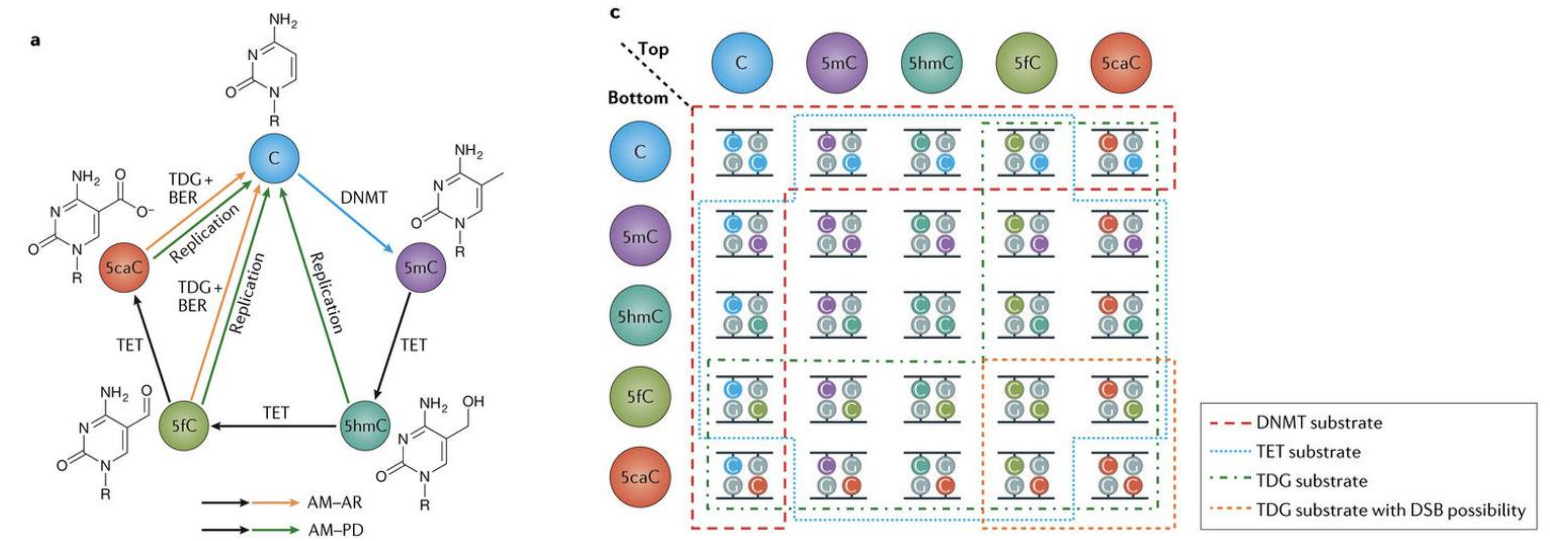
\includegraphics[width = \textwidth]{figs/5mC.png}
\end{figure}

Hay varias formas de medir la metilación en el ADN. Una técnica puede ser \textbf{afinidad por enriquecimiento con anticuerpos}. Esto es relativamente barato, pero aporta una resolución baja. Además, tiene un sesgo en cuanto a la variación del número de copias en regiones con alto contenido en GC. Se puede medir con distintos tipos de assays, pasando de arrays a nanopore. 

Hasta hace no mucho no se podía identificar a tiempo real y a nivel de moléculas únicas, la metilación de citosinas. Recientemente se consiguió hacer secuenciación single-cell para la metilación, pero todavía no está muy extendido al ser complejo. 

Dependiendo de los métodos, vamos a ir de un procesamiento de los datos bajo a complejo y cantidad de información. Las técnicas de NGS tenían un procesamiento relativamente bajo y se obtiene una gran cantidad de CpGs analizados por secuencia. Los arrays tienen un procesamiento muy complejo, y no da tanta información. No obstante, muchos datos públicos están hechos con Infinium 450K, ya que estuvo muy de moda hace 20 años. Siempre se necesita un control de muestra para saber si hay cambios entre la metilación o no. Así, se deben hacer varios experimentos. Por ejemplo, teniendo tejido normal y tumoral, en ambos se deben añadir anticuerpos, y luego hacer un control sin anticuerpo o con uno inespecífico. 

Actualmente, Infinium 450K se dejó de vender y se sustituyó por MethylationEPIC. Este kit permite identificar sitios CpG fuera de las islas de CpG, sitios metilados no CpG en células madre humanas, sitios metilados diferencialmente en tumor vs tejido normal, enhancers de FANTOM5, etc. 

La alternativa a los anticuerpos es la \textbf{técnica basada en conversión con bisulfito}, la cual tiene una resolución a nivel de nucleótido único, pero tiene un trabajo computacional intensivo. Las citosinas no metiladas se convierten en uracilos, mientras que las metiladas no se modifican. Por tanto, en una lectura de PCR, los uracilos se leen como timinas por la polimerasa. 

\begin{figure}[h]
\centering
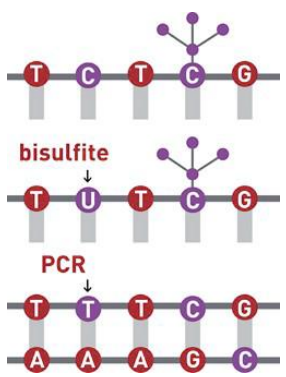
\includegraphics[width = 0.3\textwidth]{figs/bisulphite.png}
\end{figure}

Esto no deja de ser una modificación química, y se han descrito muchas otras reacciones, aunque el bisulfito sea el más habitual. Para mirar otro tipo de modificaciones, se pueden utilizar otras reacciones que produzcan otros cambios químicos en el ADN. El proceso del bisulfito no distingue entre citosinas metiladas, hidroxi-metiladas, formi-metiladas, etc. En determinados escenarios de desarrollo, experimentos de bisulfito no permite distinguir los tipos de modificación de la citosina. Esto también es importante para trabajos en tejido cerebral; para otros estudios puede no ser importante.

Hay dos protocolos de bisulfito: direccional y no direccional. Ahora se puede identificar si la lectura viene de una hebra o de otra. 

Hay dos tipos principales de alineadores. Los wild-cards reemplazan las citosinas por Y en las lecturas secuenciadas. Los alineadores de tres letras convierten la citosina en timina en las dos lecturas secuenciadas y en el genoma de referencia. 
Los wild-cards hacen alineaciones más precisas y consistentes entre réplicas, y son más eficientes en el uso de memoria y tiempos de ejecución. Pero introducen un sesgo al alza en los valores de metilación. Tras el alineamiento frente al genoma de referencia, se cuenta el número de citosinas (metiladas) y timinas (citosinas no metiladas) en la misma posición para ver el ratio. Para los wild-cards se permite el alineamiento con mismatches de Y en posiciones de C. 

Hay una herramienta llamada BioTools que tiene muchas herramientas para las ómicas. Es de la empresa Élixir, una empresa europea que representa la infraestructura de los datos. Es federado al tener distintos nodos, uno por país y tener muchas comunidades de trabajo. Mantienen el catálogo de herramientas BioTools. 

Una vez con la secuencia, el resto de los análisis son bastante triviales. Se hace lo mismo que con el resto de estudios, solo cambia el alineamiento. Se utiliza fastqc para ver cómo ha ido la secuenciación, se visualiza de distintas formas, se obtiene un score de metilación, se pueden anotar las citosinas en función de su localización genómica (región de enhancers, promotor, etc), metilación diferencial, clasificadores, etc.

Factores que afectan a la precisión de los resultados son el proceso de bisulfitado (no todas las citosinas se van a convertir en uracilo) y el alineamiento, que dependiendo del método puede ser más complejo. 

\subsubsection{Ejercicio: generación de datos sintéticos de bisulfito}
Queremos crear 150.000 lecturas direccionales de bisulphite-seq de 70 pares de base con aproximadamente 50\% CpG. 

\texttt{./Sherman -l 70 -n 150000 --genome\_folder ./ --CG 50 --CH 2 -e 0.5 > bisulphite-in-silico.txt}
